% ****** Start of file apssamp.tex ******
%
%   This file is part of the APS files in the REVTeX 4.2 distribution.
%   Version 4.2a of REVTeX, December 2014
%
%   Copyright (c) 2014 The American Physical Society.
%
%   See the REVTeX 4 README file for restrictions and more information.
%
% TeX'ing this file requires that you have AMS-LaTeX 2.0 installed
% as well as the rest of the prerequisites for REVTeX 4.2
%
% See the REVTeX 4 README file
% It also requires running BibTeX. The commands are as follows:
%
%  1)  latex apssamp.tex
%  2)  bibtex apssamp
%  3)  latex apssamp.tex
%  4)  latex apssamp.tex
%
\documentclass[%
 reprint,
%superscriptaddress,
%groupedaddress,
%unsortedaddress,
%runinaddress,
%frontmatterverbose, 
%preprint,
%preprintnumbers,
%nofootinbib,
%nobibnotes,
%bibnotes,
 amsmath,amssymb,
 aps,
%pra,
%prb,
%rmp,
%prstab,
%prstper,
%floatfix,
]{revtex4-2}
\usepackage{kotex}
\usepackage{physics}
\usepackage{graphicx}% Include figure files
\usepackage{dcolumn}% Align table columns on decimal point
\usepackage{bm}% bold math
%\usepackage{hyperref}% add hypertext capabilities
%\usepackage[mathlines]{lineno}% Enable numbering of text and display math
%\linenumbers\relax % Commence numbering lines

%\usepackage[showframe,%Uncomment any one of the following lines to test 
%%scale=0.7, marginratio={1:1, 2:3}, ignoreall,% default settings
%%text={7in,10in},centering,
%%margin=1.5in,
%%total={6.5in,8.75in}, top=1.2in, left=0.9in, includefoot,
%%height=10in,a5paper,hmargin={3cm,0.8in},
%]{geometry}

\def\rcurs{{\mbox{$\resizebox{.16in}{.08in}{
\includegraphics{ScriptR}}$}}}
\def\brcurs{{\mbox{$\resizebox{.16in}{.08in}{
\includegraphics{BoldR}}$}}}
\def\hrcurs{{\mbox{$\hat \brcurs$}}}

\begin{document}


\title{제만효과 실험 보고서}

\author{서울대학교 전기정보공학부 2018-12432 박정현}
 \email{alexist@snu.ac.kr}
\date{실험일자 : 11.06.2023}% It is always \today, today,
             %  but any date may be explicitly specified

\begin{abstract}
본 실험에서는 디락방정식을 이용해 fine structure를 계산하고 실험적으로 상대론과 양자물리의 조합이 consistent함을 간접적으로 증명한다. $10\%$이내에서 이론치와 측정값이 일치했으며 온도에 따른 실험 장비의 변화, spectrum의 broadening에 의한 정확도 저하 등과 같은 실험의 한계점을 제시한 뒤 새로운 장비와 다른 방법의 실험 방법을 제시하였다.
\end{abstract}

%\keywords{Suggested keywords}%Use showkeys class option if keyword
                              %display desired
\maketitle

%\tableofcontents

\section{\label{sec:level1}Introudction}
양자물리는 뉴턴의 고전물리에 비해 짧은 기간 연구되었지만 매우 깊이 연구된 학문이다. 양자물리의 역사에서 여러가지의 사건들이 나타나 물리학자들에게 충격을 주었으며 새로운 breakthrough를 만드는데 큰 역할을 하였다. 특히 1940년대부터 1970년 사이에는 양자물리와 상대론을 조합하려는 여러 시도들이 있었으며 디락은 디락방정식을 통해 상대론과 양자물리가 조합된 식을 제시하였고 이후에 여러 물리학자들은 이론적인 예측과 실험이 일치함을 확인하였다. 이러한 학문의 발전을 통해 원자들의 내부 구조는 더 정확히 분석되었으며 물리학도로서 알아야할 중요한 역사라고 할 수 있다. 본 실험에서는 디락 방정식을 통해 fine strucuture를 계산하고 수은의 내부 전자 전이를 빛의 간섭을 통해 측정하여 상대론과 양자물리가 조합된 디락방정식이 consistent함을 간접적으로 증명하고 양자물리와 상대론에 대한 이해도를 높인다.
 
\subsection{\label{sec:level2}Fine Structure}
수소원자의 슈뢰딩거 방정식은 아래와 같다.
\begin{align}
	H\psi &= -\frac{\hbar^{2}}{2m}\nabla^{2}\psi - \frac{1}{4\pi \epsilon_{0}}\frac{e^{2}}{r}\psi
\end{align}
이 때 수소원자의 해는 아래와 같이 나타난다.
\begin{align}
	\psi(r,\theta,\phi) = R_{nl}(r)\Theta_{l}(\theta)\Phi_{m}(\phi)
\end{align}
상대론을 고려하지 않는 경우 동일한 양자수 n에 대해서 수소원자는 모두 동일한 에너지를 가진다.[1] 즉, degnerate된 상태로 존재한다. 하지만 상대론을 고려하여 수소원자를 풀게 되면 양자수 l에 대한 degenerate는 깨지게 된다. 디락 방정식을 다른 좌표계로 변환하여 (\ref{eq:perfecteq})와 같이 정확한 해를 계산할수 있다.

\begin{widetext}
\begin{align}
	E_{j,n} &= -m_{e}c^{2}\left[ 1- \left( 1 + \left[ \frac{\alpha}{n-j-1/2+\sqrt{(j+1/2)^{2}-\alpha^{2}}} \right] \right)^{-1/2} \right]\label{eq:perfecteq}
\end{align}
\end{widetext}

하지만 디락방정식의 해를 정확하게 계산하는 것은 모든 원자에 적용이 불가능할 뿐더라 물리적 의미를 파악하는데 어려움이 따른다. 이와 반대로 디락방정식에서 시작하여 작은 perturbation들로 근사하여 항들을 직접 계산하면 물리적 의미를 더 깊게 이해할 수 있을 것이다. 디락 방정식은 (\ref{eq:dirac})와 같다.

\begin{align}
	(E+c\vec{\alpha}\cdot\vec{p}+\beta mc^{2})\psi = 0\label{eq:dirac}
\end{align}

여기서 $\alpha$와 $\beta$는 Dirac-Pauli representation을 따른다. $\psi$는 4개의 항을 가지는 vector이며 양의 질량을 가진 해만을 고려하면 식은 (\ref{eq:dirac2})와 같아진다. 단, $\pi = \vec{p}-q\vec{A}$, $E' = E-mc^{2}$이다. 

\begin{align}
	\begin{aligned}\label{eq:dirac2}
		(E'+2mc^{2}-q\phi)\psi_{1} + c\pi\cdot\sigma\psi_{2} &=0\\
		(E'-q\phi)\psi_{2}+c\pi\cdot\sigma\psi_{1} &= 0
	\end{aligned}
\end{align}

$\psi_{2}$에 대해서 풀면 식은 (\ref{eq:dirac3})와 같아진다. 

\begin{align}
	E'\psi_{2} &= q\phi\psi_{2}+ c\pi\cdot\sigma\frac{1}{E'+2mc^{2}-q\phi}\pi\cdot\sigma\psi_{2}\label{eq:dirac3}
\end{align}

$\phi =0$일때  1차항에 대해서 아래와 같이 근사된다.

\begin{align}
	E' &= \frac{1}{2m}(\pi\cdot\sigma)^{2}\\
	&= \frac{1}{2m}\pi^{2}-\frac{\hbar q}{2m} \sigma \cdot \vec{B}\\
	&= \frac{p^{2}}{2m} - \frac{q}{2m}\vec{L}\cdot\vec{B}+\frac{q^{2}}{2m}A^{2}-\frac{2q}{2m} \vec{S}\cdot \vec{B}\\
	&= \frac{p^{2}}{2m} -\frac{q}{2m}(\vec{L}+2\vec{S})\cdot\vec{B}+\frac{q^{2}}{2m}A^{2}\label{eq:rel_zeeman}
\end{align}

따라서 외부자기장에 대해서 $\frac{q}{2m}(\vec{L}+2\vec{S})\cdot\vec{B}$만큼의 perturbation이 생김을 알 수 있다. $\phi =0$, $A=0$일 때 위치에 대한 미분연산자임을 이용하면 운동량 연산자는 1차항에 대해서 식(\ref{eq:final_dirac})와 같이 근사된다.
\begin{align}
	E' &= \frac{p^{2}}{2m}+U -\frac{p^{4}}{8m^{3}c^{2}}-\frac{i\hbar}{4m^{2}c^{2}}\nabla U \cdot\vec{p}+\frac{\hbar}{4m^{2}c^{2}}\sigma \cdot[\nabla U \times \vec{p}]\\
	&=\left(\frac{p^{2}}{2m}+U\right) -\frac{p^{4}}{8m^{3}c^{2}}-\frac{\hbar^{2}}{4m^{2}c^{2}}\frac{dU}{dr}\partial_{r} + \frac{1}{2m^{2}c^{2}}\frac{1}{r}\frac{dU}{dr}\vec{L}\cdot\vec{S}\label{eq:final_dirac}
\end{align}

첫번째 항은 nonrelativistic effect, 두번째 항은 relativistic effect, 세번째 항은 darwin term, 그리고 마지막은 LS coupling에 해당한다.

\subsubsection{\label{sec:level2}Relativistic Effect}
상대적으로 움직이는 전하가 만드는 자기장에 의해 분리된 에너지인 spin-orbit coupling, 그리고 상대론적인 에너지 $E=\sqrt{p^{2}c^{2}+m^{2}c^{4}}$을 1차 근사 하여 perturbation을 계산하여도 1차항에서 동일한 결과를 나타낸다.[1] 상대론에 의한 perturbation은 $\sqrt{p^{2}c^{2}+m^{2}c^{4}} \simeq \frac{p^{2}}{2m} - \frac{p^{4}}{8m^{3}c^{2}}$에서 운동량의 4차항에 해당한다. $E_{n}\psi_{n} = (\frac{p^{2}}{2m}+V)\psi_{n}$임을 이용하면 perturbation에 의한 에너지 차이를 계산하면 아래의 식으로 정리된다.

\begin{align}
	\Delta^{1}_{n,l,rel} &= - \bra{n,l}\frac{p^{4}}{8m^{3}c^{2}}\ket{n,l}\\
	&= \frac{1}{8m^{3}c^{2}}\bra{n,l}p^{4}\ket{n,l}\\
	&= \frac{1}{2mc^{2}}\bra{n,l}E_{n}^{2} + 2E_{n}\frac{1}{4\pi \epsilon_{0}}\frac{e^{2}}{r}+ \frac{1}{16\pi^{2} \epsilon_{0}^{2}}\frac{e^{4}}{r^{2}}\ket{n,l}\\
	&= \frac{E^{2}_{n}}{2mc^{2}}\left( \frac{4n}{l+1/2}-3 \right)
\end{align}

\subsubsection{\label{sec:level2}LS Coupling}
고전물리학에서 전자가 원자핵 주변을  공전한다고 고려하고 움직이는 전하의 좌표계로 로렌츠 변환을 하면 핵에 의한 전기장은 자기장으로 변환 된다. 앞서 계산한 디락방정식을 4개의 항에 대해서 계산하면 전자는 $+1/2, -1/2$의 두가지 스핀을 가진다. 이 때 전자의 쌍극자 모멘트를 스핀을 이용해 나타내면 아래와 같이 나타난다.

\begin{align}
	\vec{\mu} = -g_{s}\mu_{B}\frac{\vec{S}}{\hbar}
\end{align}

$g_{s}$는 전자의 g-factor, 그리고 $\mu_{B}$는 Bohr magneton에 해당하는 값이다. 디락방정식에 따르면 $g_{s}=2$라는 정수 값을 가진다. 하지만 quantum field thoery에 따라 전자가 방출하는 광자를 다시 흡수하는 과정을 모두 고려하여 $g_{s}$값을 계산하면 $g_{s} = 2.0023$이라는 값을 가진다. 디락방정식에서 나타나는 이러한 차이는 lamb shift으로도 관측되며 더 정확한 수치를 계산하려면 QFT를 고려하여 계산하여야 한다.[7] 하지만 본 실험에서는 이러한 효과까지 모두 측정하는 것이 목적이 아니므로 해당 수치들은 무시한다.

원자핵에 의한 전기장을 회전 좌표계로 변환하면 아래의 식을 만족한다.[3]
\begin{align}
	\vec{B} &= -\frac{\vec{v}\times\vec{E}}{c^{2}}
\end{align}

$\vec{p} = m\vec{v}$, $\vec{L} = \vec{r}\times{p}$임을 이용하면 자기장은 아래와 같이 나타난다.

\begin{align}
	\vec{B} &= \frac{1}{mec^{2}}\frac{1}{r}\frac{\partial U}{\partial r} \vec{L}
\end{align}

따라서 LS coupling 항은 아래와 같다.
\begin{align}
	\frac{1}{m^{2}c^{2}}\frac{1}{r}\frac{dU}{dr}\vec{L}\cdot\vec{S}
\end{align}

고전적으로 계산한 결과와 디락방정식에서 유도된 (\ref{eq:final_dirac})와 2배 차이가 나는데 이거은 thomas precision을 고려하지 않아 발생한 현상이다. Thomas precision을 고려하면 LS coupling에 의한 perturbation은 아래와 같아진다.

\begin{align}
	\Delta^{1}_{n,l,LS} &= \left<\frac{\mu_{B}}{\hbar m e c^{2}}\frac{1}{r}\frac{\partial U}{\partial r}\vec{L}\cdot\vec{S}\right>\\
	&=\frac{E_{n}^{2}}{mc^{2}}n\frac{j(j+1)-l(l+1)-\frac{3}{4}}{l(l+1/2)(l+1)}
\end{align}


\subsubsection{\label{sec:level2}Total Energy}
Darwin Term은 classical concept에 명확하게 일대일 대응이 되는 항이 아니다. 하지만 electron의 random한 운동으로 인해 만들어지는 퍼텐셜의 randomness로 이해할 수 있으며 이를 이용해 에너지를 계산하면 $\psi(0)$의 제곱에 비례하는 항이 계산된다. 이를 모두 고려하여 에너지를 계산하면 아래와 같다.
\begin{align}
	E_{n^{2S+1}L_{J}} &= -\frac{2\alpha^{2}}{2n^{2}}mc^{2} + \alpha^{4}mc^{2}\left[\frac{3}{8n^{4}}-\frac{1}{n^{3}(2j+1)}\right]
\end{align}

여기서 $n^{2S+1}L_{J}$은 term symbol로 원자내의 전자의 고유상태를 나타내는 부호이다.

\subsection{\label{sec:level2}Spin of photon}
단위벡터 $\hat{r}$은 아래와 같이 나타난다.

\begin{align}
	\hat{r} &= \sqrt{\frac{4\pi}{3}}\left(Y_{1,-1}\frac{\hat{e}_{1}+i\hat{e}_{2}}{\sqrt{2}}+Y_{1,0}\hat{e}_{3}+Y_{1,1}\frac{\hat{e}_{1}-i\hat{e}_{2}}{\sqrt{2}}\right)
\end{align}

Electric field가 양자화 되지 않은 semiclassical 영역에서 전기장 속에서의 원자의 광자 방출 속도는 다음의 식에 비례한다.

\begin{align}
	\Gamma &\simeq eE_{0}^{2} \abs{\bra{2}\vec{r}\cdot\vec{e}_{electric}\ket{1}}
\end{align}

전기장의 단위벡터는 아래와 같이 나타난다.

\begin{align}
	\vec{e}_{electric} &= \left(A_{\sigma -}\frac{\hat{e}_{1}+i\hat{e}_{2}}{\sqrt{2}}+A_{\pi}\hat{e}_{3}+A_{\sigma +}\frac{\hat{e}_{1}-i\hat{e}_{2}}{\sqrt{2}}\right)
\end{align}

따라서 원자의 스핀이 $\Delta m = \pm 1$만큼 변화한 경우 자기장에 수직한 $\frac{\hat{e}_{1}+i\hat{e}_{2}}{\sqrt{2}}$,$\frac{\hat{e}_{1}-i\hat{e}_{2}}{\sqrt{2}}$ 편광 성분을 가진 광자가 방출된다. 반면에 원자의 스핀이 $\Delta m = 0$으로 변화하지 않은 경우 자기장에 수직한 방향으로 편광된 광자가 방출된다. 이것은 각각 광자의 스핀에 대응된다. 따라서 편광장치를 자기장과 평행한 방향으로 설치한 경우 $\Delta m = 0$에서 전이하여 방출된 광자만 관측된다.[8]

\subsection{\label{sec:level2}Zeeman Effect}
식 (\ref{eq:rel_zeeman})에서 계산한 것과 같이 외부에서 자기장이 가해진 경우 에너지는 자기장과 각운동 모멘텀, 스핀 모멘텀에 내적한 만큼의 perturbation이 발생한다. 이러한 현상을 zeeman effect라고 하며 해당 에너지는  $n^{2S+1}L_{J}$에 대해서 z방향 각운동량 연산자가 모두 good quantum number이므로 아래와 같이 표현된다.

\begin{align}
	E_{ZE} &= g_{J}\mu_{B}BM_{J}\\
	g_{J} &= \frac{3}{2} + \frac{S(S+1) - L(L+1)}{2J(J+1)}
\end{align}

원자가 다른 level로 전이하는 경우 selection rule에 의해 $\Delta L = \pm 1$, $\Delta m = 0, \pm1$을 만족해야 한다. 따라서 수은원자에서 $^{3}S_{1} \rightarrow ^{3}P_{2}$로 전이하는 경우 Fig.\ref{fig:Mercury}와 같은 전이만이 가능하다. 따라서 가해준 자기장에 수직한 편광판을 설치하는 경우 3개의 split 된 광자를 관측할 수 있다.[2] 

\begin{figure}[htbp]
	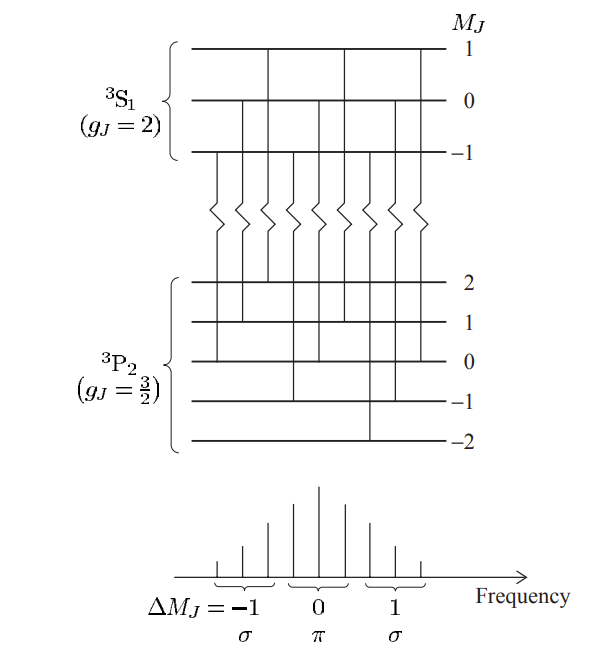
\includegraphics[width = 0.95\linewidth]{Mercury.png}% Here is how to import EPS art
	\caption{\label{fig:Mercury}수은 원자의 에너지 전이}
\end{figure}

광자의  에너지가 $hc/\lambda$임을 이용하면 $\Delta m = \pm 1$ 원자 전이에서 방출된 광자의 파장 차이는 아래와 같이 나타난다.

\begin{align}
	\Delta \lambda &= \frac{B\mu_{B}\lambda^{2}}{hc}
\end{align}

두 광자가 Fig.\ref{fig:Fabry}와 같은 Fabry-Perot Interferometry를 지나가 초점거리 $f$의 렌즈에 의해 상이 맺히면 근축근사를 적용했을 때 아래의 식이 성립한다. 

\begin{figure}[htbp]
	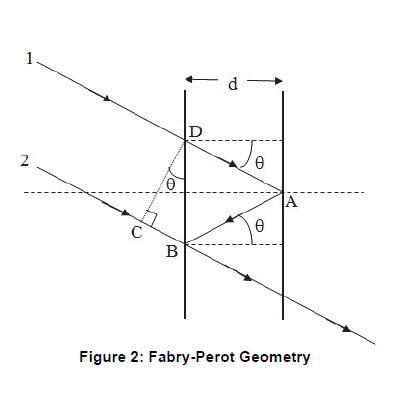
\includegraphics[width = 0.95\linewidth]{Fabry.png}% Here is how to import EPS art
	\caption{\label{fig:Fabry}Fabry-Perot Interferometry}
\end{figure}

\begin{align}
	2d\left(1-\frac{\theta^{2}_{k}}{2} \right) &= (n-k)\lambda\\
	&2d\left(1-\frac{R^{2}_{k}}{2f^{2}} \right)
\end{align}

따라서 아래의 식이 성립한다.

\begin{align}
	\frac{d}{f^{2}}(R_{k+}^{2}-R_{k-}^{2}) &=(n-k)(\Delta\lambda)\\
	&= (n-k)\frac{B\mu_{B}\lambda^{2}}{hc}
\end{align}

따라서 k=0일 때 반지름을 $R_{0}$으로 둘 경우 아래의 식이 성립한다.
\begin{align}
	\mu_{B} &= \left( \frac{C_{0}hc}{2dB}\right)(R_{k+}^{2}-R_{k-}^{2})\\
	C_{0} &= \frac{d}{f^{2}\lambda}\\
	&= \frac{k}{R_{k}^{2}-R_{0}^{2}}
\end{align}

\section{\label{sec:level1}Experimental}
본 실험에서는 Fig.\ref{fig:SE9654}의 PASCO의 SE-9654를 이용하여 실험을 수행하였다. 솔레노이드 내에 수은 원자를 배치하였으며 솔레노이드를 통해 1T가량의 자기장을 인가할 수 있다. 이 때 방출된 광자들은 편광판, 렌즈를 지난 후 CCD 카메라에 도달하여 interference를 형성한다. CCD카메라와 PC를 연결하여 PASCO Capstone 프로그램을 통해 원형 interference의 반지름을 측정하고 이후 전류값을 $4.5, 5.0, 5.5A$에서 각각의 반지름을 다시 측정한다.

\begin{figure}[htbp]
	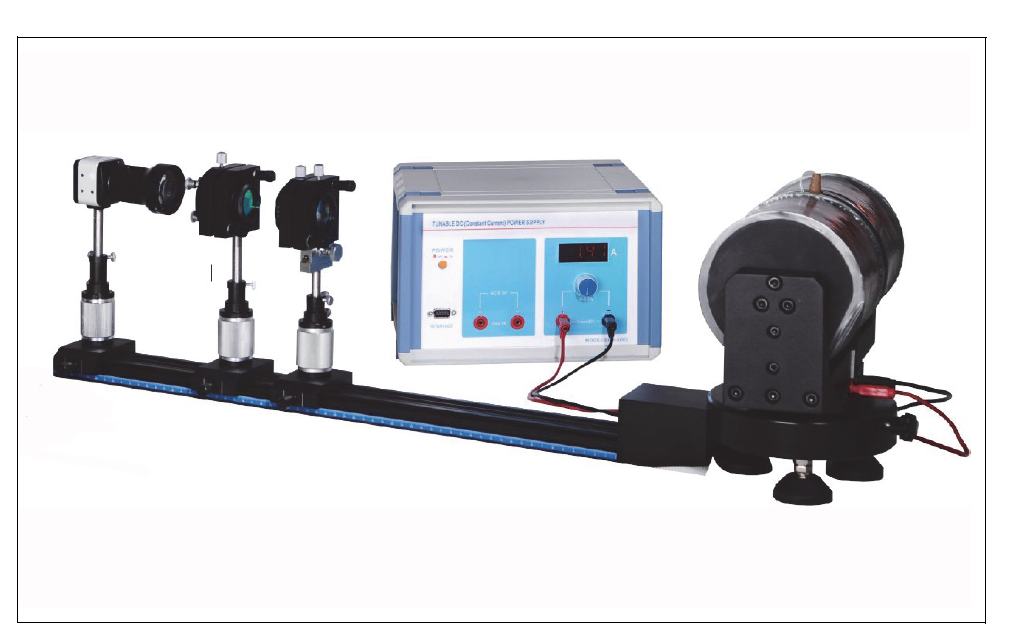
\includegraphics[width = 0.95\linewidth]{SE9654.png}% Here is how to import EPS art
	\caption{\label{fig:SE9654}SE-9654}
\end{figure}


\section{\label{sec:level1}Data \& Result}
자기장이 없는 경우 측정된 반지름은 Tab.\ref{tab:Cmes}와 같다. 이를 이용해 fitting 하면 Fig.\ref{fig:Cfig}와 같으며 $C_{0}$의 값은 $6.422\pm 0.642 $이다. 여기서 오차는 원 반지름의 broadening에 의한 것이다.

\begin{table}[]
\begin{tabular}{c|c} \hline \hline
k & R[m]  \\ \hline
0 & $0.3326\pm0.05$ \\  
1 & $0.5196\pm0.05$ \\  
2 & $0.6528\pm0.05$ \\  
3 & $0.7606\pm0.05$ \\  
4 & $0.8562\pm0.05$ \\  
5 & $0.9461\pm0.05$ \\  \hline \hline 
\end{tabular}
\caption{\label{tab:Cmes}$C_{0}$측정을 위한 반지름 측정}
\end{table}

\begin{figure}[htbp]
	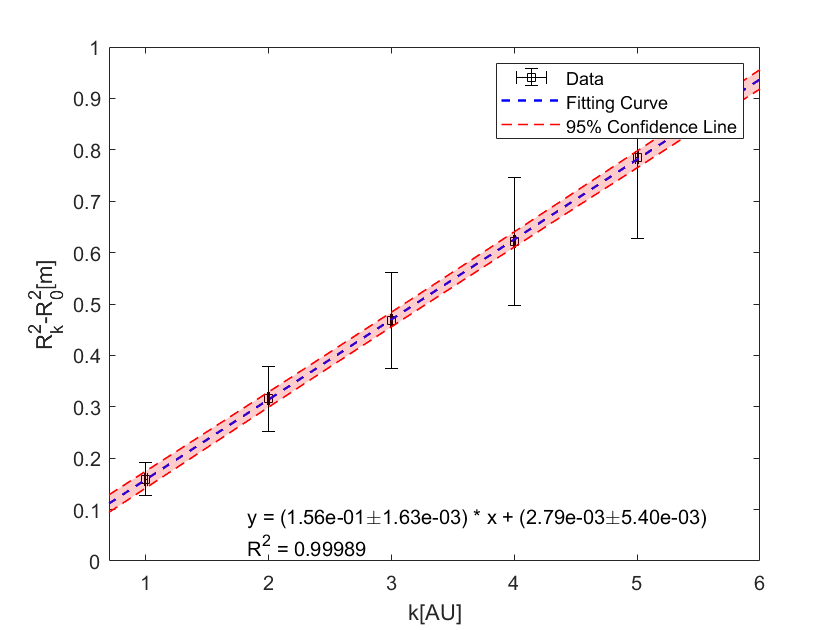
\includegraphics[width = 0.95\linewidth]{Cfig.png}% Here is how to import EPS art
	\caption{\label{fig:Cfig}k에 따른 $R_{k}^{2}-R_{0}^{2}$}
\end{figure}

앞서 구한 $C_{0}$값을 이용하여 각각의 전류에서 측정한 bohr magneton은 각각 Tabs.\ref{tab:bohr1},\ref{tab:bohr2},\ref{tab:bohr3}와 같다.
\begin{table}[]
\begin{tabular}{c|c|c|c} \hline \hline
k & $R_{+}[m]$ & $R_{-}[m]$ & $\mu_{B}[J/T]$ \\ \hline
0&	$0.3454\pm0.05$&	$0.2957\pm0.05$&	$9.52\times10^{-24}$\\
1&	$0.5262\pm0.05$&	$0.4932\pm0.05$&	$1.00\times10^{-23}$\\
2&	$0.6569\pm0.05$&	$0.6358\pm0.05$&	$8.15\times10^{-24 }$\\ \hline \hline 
\end{tabular}
\caption{\label{tab:bohr1}I=4.5A에서 측정한 반지름(B=1.070T)}
\end{table}

\begin{table}[]
\begin{tabular}{c|c|c|c} \hline \hline
k & $R_{+}[m]$ & $R_{-}[m]$ & $\mu_{B}[J/T]$ \\ \hline
0&	$0.3503\pm0.05$&	$0.2992\pm0.05$&	$9.61\times10^{-24}$\\
1&	$0.5355\pm0.05$&	$0.4969\pm0.05$&	$1.15\times10^{-23}$\\
2&	$0.6650\pm0.05$&	$0.6325\pm0.05$&	$1.22\times10^{-23}$\\ \hline \hline 
\end{tabular}
\caption{\label{tab:bohr2}I=5.0A에서 측정한 반지름(B=1.105T)}
\end{table}

\begin{table}[]
\begin{tabular}{c|c|c|c} \hline \hline
k & $R_{+}[m]$ & $R_{-}[m]$ & $\mu_{B}[J/T]$ \\ \hline
0&	$0.3642\pm0.05$&	$0.3047\pm0.05$&	$1.10\times10^{-23}$\\
1&	$0.5384\pm0.05$&	$0.5023\pm0.05$&	$1.04\times10^{-23}$\\
2&	$0.6670\pm0.05$&	$0.6367\pm0.05$&	$1.10\times10^{-23}$\\ \hline \hline 
\end{tabular}
\caption{\label{tab:bohr3}I=5.5A에서 측정한 반지름(B=1.153T)}
\end{table}

따라서 측정된 bohr magneton은 $(1.04\pm 0.2 )\times10^{-23}[J/T]$으로 이론 값인 $\frac{e\hbar}{2m}=9.27\times 10^{-24}[J/T]$와 약 $10\%$ 오차 내에서 일치한다. 따라서 상대론적으로 양자역학을 기술하는 것이 consistent함을 간접적으로 보였다.

\section{\label{sec:level1}Discussion}
본 실험에서는 디락방정식으로부터 유도된 해밀토니안으로부터 에너지를 계산하였으며 이러한 에너지를 기반으로 측정한 간섭무늬가 이론적인 예측과 일치함을 확인하였다. 하지만 실험에서 반지름의 width가 너무 커 측정 기준이 모호하였으며 이론적인 값보다 더 큰 값이 측정되었다. Fabry-perot 간섭계 사이의 거리는 금속의 열팽창 계수에 의해 온도에 따라 일정하지 않을 것이다. 특히 낮은 온도에서 더 작은 d값을 가져 이론적인 예측치보다 더 큰 값이 측정되도록 만들 것이다. 이를 보완하기 위해 일정한 온도에서 실험을 진행하거나, 간섭계 사이의 거리를 보정하는 piezo device를 PI control하는 방법이 있을 것이다.

더 정밀한 레이저를 이용해 수은원자를 모두 $^{3}P_{2}$ state로 초기화 한 이후  rabi rotation하며 각각의 시간에서 state의 확률을 측정하는 방법 또한 있을 것이다. 이러한 실험을 진행하기 위해서는 정밀한 time resolution을 가진 장비가 필요하며 FPGA와 같은 장비를 활용해야 할 것이다. 실제로 양자정보 실험에서는 Xilinx 사의 FPGA를 이용하여 원자의 state를 정확하게 control한다. 대표적인 장비의 예로는 M-Labs의 Artiq[10], 그리고 Sandia 연구소의 RFSoC 장비 및 프로그램 QSCOUT이 있다.[11] Sandia 연구소의 RFSoC의 경우 Yb원자를 다른 phonon state를 변화시키지 않기 위해 FM modulation된 전자기파를 AOM을 통해 369nm레이저에 mixing을 한후 Yb원자를 raman transition한다. 따라서 정확한 bohr magneton을 측정하기 위한 장비는 충분히 존재하며 오로지 금전적인 원인을 제외하면 현재까지 개발된 장비들에 기반하면 기술적인 측면에서 측정하지 못할 이유는 없다.

물리적인 오차 원인으로는 원자의 decay rate로 은한 frequency shape의 boradening이 있다. 원자의 spontaneous decay,  non-radiative decay와 같은 decay는 frequency space에서 peak의 width를 만든다. 특히 원자의 전이 spectrum은 lorentzian을 따르며[12] 각각의 decay가 합쳐진 width가 나타난다. thermal noise에 의한 non-radiative decay rate를 감소시키기 위해 극저온에서 실험을 진행할 수 도 있을 것이다. 혹은 원자분수를 이용해 ramsey fringe를 측정하면 frequency width보다 작은 frequency resolution으로 원자의 reonance frequency를 측정할 수 있다.[4] 이를 활용하여 mercury의 resonance frequency를 측정한 후 bohr magneton을 더 정확히 측정할 수 있을 것이다.

\section{\label{sec:level1}Reference}
[1] Griffiths, D. J. (2017, January 1). Quantum Mechanics in Three Dimensions. In \textit{Introduction to Quantum Mechanics}. (pp. 131-154). Cambridge University Press.

[2] Foot, C. (2005, January 1). Fine structure in the LS-coupling scheme. In \textit{Atomic Physics} (pp. 90–92). Oxford University Press.

[3] Griffiths, D. J. (2014, January 13). Relativistic Electrodynamics. In \textit{Introduction to Electrodynamics}. Pearson Higher Ed. ( p. 559)

[4] Foot, C. (2005, January 1). The interaction of atoms with radiation. In \textit{Atomic Physics} (p. 134). Oxford University Press.

[5] 제원호, Atomic Physics, 2nd Semester, 2019

[6] Foot, C. (2005, January 1). Fine structure in the LS-coupling scheme. In \textit{Atomic Physics} (p. 92). Oxford University Press.

[7] Foot, C. (2005, January 1). The hydrogen atom. In \textit{Atomic Physics} (pp. 40–41). Oxford University Press.

[8]  Foot, C. (2005, January 1). The hydrogen atom. In \textit{Atomic Physics} (pp. 30–31). Oxford University Press.

[10] M-Labs. (n.d.). M-Labs. https://m-labs.hk/experiment-control/artiq/

[11] Clark, S. M., Lobser, D., Revelle, M. C., Yale, C. G., Bossert, D., Burch, A. D., Chow, M. N., Hogle, C. W., Ivory, M., Pehr, J., Salzbrenner, B., Stick, D., Sweatt, W., Wilson, J. M., Winrow, E., \& Maunz, P. (2021). Engineering the Quantum Scientific Computing Open User Testbed. \textit{IEEE Transactions on Quantum Engineerin}g, 2, 1–32. https://doi.org/10.1109/tqe.2021.3096480

[12]  Foot, C. (2005, January 1). The interaction of atoms with radiation. In \textit{Atomic Physics} (p. 139). Oxford University Press.
\end{document}
%
% ****** End of file apssamp.tex ******
